%%%%%%%%%%%%%%%%%%%%%%%%%%%%%%%%%%%%%
% Read the /ReadMeFirst/ReadMeFirst.tex for an introduction. Check out the accompanying book "Better Books with LaTeX" for a discussion of the template and step-by-step instructions. The template was originally created by Clemens Lode, LODE Publishing (www.lode.de), mail@lode.de, 8/17/2018. Feel free to use this template for your book project!
%%%%%%%%%%%%%%%%%%%%%%%%%%%%%%%%%%%%%

% Selecting document class scrbook to be in the two-page mode and accommodate for the binding of a printed book.
% The bibliography receives an entry in the table of contents but no number.
\documentclass[pagesize=auto,bibliography=totocnumbered]{scrbook}
\title{Clemens Lode's LaTeX Book Template}

% activate babelEN
\usepackage[american]{babel}


% add a list of words to enforce a certain hyphenation for them.
\usepackage{xspace}
\usepackage{hyphenat}
\hyphenation{}

% load additional LaTeX libraries.
% Activate warnings about outdated / invalid packages
\RequirePackage[l2tabu, orthodox]{nag}

% Provide full error messages
\errorcontextlines 10000

% Enables checking if XeLaTeX is used.
\usepackage{ifxetex}

% Load additional packages for the PDF output
\ifxetex
	% adjusting figures to fit into the width of a page.
	\usepackage{adjustbox}
    
	% Fancy lines for chapters and end of sections.
	\usepackage{psvectorian}
\else
	% Ignore adjustbox commands (HTML files do not have a width).
	\newcommand{\adjustbox}[2][]{#1}

	% Ignore psvectorian lines.
	\newcommand{\psvectorian}[2][]{}
\fi

% Translate horizontal rule and emdash into hrule / "---"
\ifx\HCode\undefined 
	\def\myrule{\hrule}
	\newcommand{\emdash}[1][]{\hspace{0pt}---\hspace{0pt}}%       
\else
	\def\myrule{\HCode{<hr style="clear: both" />}}
	\def\emdash{\HCode{&\#8212;}}
    \renewcommand\newpage[1][]{\HCode{<mbp:pagebreak />}}
\fi


% load our own packages
% Fix PDF creation
\ifxetex
	\let\pdfstrcmp\strcmp
\fi

% this is the macro to define phrases in two languages:
\newcommand{\babelDE}[1]{\ifnum\pdfstrcmp{\languagename}{ngerman}=0 {#1}\fi}
\newcommand{\babelEN}[1]{\ifnum\pdfstrcmp{\languagename}{american}=0 {#1}\fi}

% allow hyphenation recommendation for LaTeX with "=
\useshorthands{"}
\addto\extrasenglish{\languageshorthands{ngerman}}

% Rename the table of contents depending on the used language.
\babelDE{\renewcommand{\contentsname}{Inhaltsverzeichnis}}
\babelEN{\renewcommand{\contentsname}{Table of Contents}}


% Set up bibliography.

% Advanced handling of quotation marks -> important for bibliography.
\usepackage{csquotes}

\ifxetex
% See https://www.ctan.org/pkg/biblatex for documentation.
	\usepackage[backend=bibtex,style=authortitle,sortlocale=de_DE,natbib=true]{biblatex}
	\babelDE{\addbibresource[datatype=bibtex]{bibliography/german.bib}}
	\babelEN{\addbibresource[datatype=bibtex]{bibliography/english.bib}}
\else
	\usepackage{natbib}
	\usepackage{usebib}
	\babelDE{\bibinput{bibliography/german}}
	\babelEN{\bibinput{bibliography/english}}

	% \citetitle does not work with natbib / pdfLaTeX -> translate into \usebibentry
	\newcommand{\citetitle}[2][]{\textit{\usebibentry{#2}{title}}}
\fi

% Set bibliography to footnote size
\renewcommand{\bibfont}{\footnotesize}

% Write the name of a referenced section or chapter label with \nameref{label}.
\usepackage{nameref}
% Select a book format

%\usepackage[paperwidth=12.5cm,  paperheight=19.0cm, inner=0.80in, outer=0.3in, top=0.7in, bottom=0.5in]{geometry}
%\usepackage[paperwidth=13.0cm,  paperheight=19.0cm, inner=0.80in, outer=0.3in, top=0.7in, bottom=0.5in]{geometry}
%\usepackage[paperwidth=12.85cm, paperheight=19.84cm, inner=0.80in, outer=0.3in, top=0.7in, bottom=0.5in]{geometry}
%\usepackage[paperwidth=5in,  paperheight=8in, inner=0.80in, outer=0.3in, top=0.7in, bottom=0.5in]{geometry}
\usepackage[paperwidth=5.25in,  paperheight=8in, inner=0.80in, outer=0.3in, top=0.7in, bottom=0.5in]{geometry}
%\usepackage[paperwidth=13.34cm, paperheight=20.32cm, inner=0.80in, outer=0.3in, top=0.7in, bottom=0.5in]{geometry}
%\usepackage[paperwidth=14.8cm,  paperheight=21.0cm, inner=0.80in, outer=0.3in, top=0.7in, bottom=0.5in]{geometry} % DinA5
%\usepackage[paperwidth=13.5cm,  paperheight=21.5cm, inner=0.80in, outer=0.3in, top=0.7in, bottom=0.5in]{geometry}
%\usepackage[paperwidth=13.97cm, paperheight=21.59cm, inner=0.80in, outer=0.3in, top=0.7in, bottom=0.5in]{geometry}
%\usepackage[paperwidth=15.24cm, paperheight=22.86cm, inner=0.80in, outer=0.3in, top=0.7in, bottom=0.5in]{geometry}
%\usepackage[paperwidth=15.6cm,  paperheight=23.39cm, inner=0.80in, outer=0.3in, top=0.7in, bottom=0.5in]{geometry}
%\usepackage[paperwidth=19.05cm, paperheight=23.5cm, inner=0.80in, outer=0.3in, top=0.7in, bottom=0.5in]{geometry}
%\usepackage[paperwidth=16.99cm, paperheight=24.41cm, inner=0.80in, outer=0.3in, top=0.7in, bottom=0.5in]{geometry}
%\usepackage[paperwidth=18.9cm,  paperheight=24.61cm, inner=0.80in, outer=0.3in, top=0.7in, bottom=0.5in]{geometry}
%\usepackage[paperwidth=17.78cm, paperheight=25.4cm, inner=0.80in, outer=0.3in, top=0.7in, bottom=0.5in]{geometry}
%\usepackage[paperwidth=20.32cm, paperheight=25.4cm, inner=0.80in, outer=0.3in, top=0.7in, bottom=0.5in]{geometry}
%\usepackage[paperwidth=21.59cm, paperheight=27.94cm, inner=0.80in, outer=0.3in, top=0.7in, bottom=0.5in]{geometry}




% Sets the font specifications for the chapter lead-in and title.
\newcommand{\chapterLeadinFont}{\Large}
\newcommand{\chapterTitleFont}{\Huge \MakeUppercase }
%
% Lengths used in the chapter title page setup. You can change the values I gave these using the "setlength" commands immediately following the length definitions. Most of these interact with each other. For example, increasing one of the gaps between the bounding rectangles decreases the maximum title width.
%
% The next three lengths adjust the size of the bounding rectangles on chapter title pages by decreasing the lengths of their sides. Increasing these lengths make the rectangles smaller. These rectangles are always centered in the text area so they should adjust to changes in your margins and paper size. The default, outer rectangle (0pt) lies on the margin. All of these lengths should be greater than or equal to zero.
\newlength{\outerRec}\setlength{\outerRec}{0pt}
\newlength{\middleRec}\setlength{\middleRec}{2pt}
\newlength{\innerRec}\setlength{\innerRec}{12pt}
%
% The next three lengths set the edge widths of the rectangles. I did not think these and the previous lengths should interact, so, if you increase these, you may need to adjust the above; otherwise, the edges of two adjacent rectangles may overlap.
\newlength{\outerLineWidth}\setlength{\outerLineWidth}{.5pt}
\newlength{\middleLineWidth}\setlength{\middleLineWidth}{.5pt}
\newlength{\innerLineWidth}\setlength{\innerLineWidth}{.5pt}
%
% Remark: You can comment one of the \draw commands in the code that follows if you want two rectangles. You can also give middle and inner lengths above the same values. 
%
% The next length sets both the left and right distances between the inside of the edge of the inner rectangle and the maximum chapter title width. A positive value ensures that the chapter title lies inside the inner rectangle. If you set this length to 0pt, a longer chapter title may touch the left and right edges of the inner rectangle.
\newlength{\adjustTitleWidth}\setlength{\adjustTitleWidth}{.8cm}
%
% The next lengths, used in the \titlespacing command, set horizontal and vertical title information distances.
\newlength{\leftMar}\setlength{\leftMar}{0pt}% Increases the left margin of the title. Normally, you should not adjust this length.
\newlength{\beforeSep}{\setlength{\beforeSep}{45pt}}% Sets the vertical between the top margin, not the inner rectangle, and the chapter lead-in.
\newlength{\spaceToRule}\setlength{\spaceToRule}{.45cm}% Set vertical spacing between chapter lead-in and the rule. 
\newlength{\spaceAfterRule}{\setlength{\spaceAfterRule}{.75cm}}% Sets the vertical spacing between the rule and the chapter title.
%
% The next length deals with the special chapter titles "Contents" and "Bibliography". It increases the distance between the upper edge of the inner rectangle and the title text.
\newlength{\specialMargin}\setlength{\specialMargin}{3.4cm}
%
\newlength{\topSep}\setlength{\topSep}{0cm}% Sets the vertical space between the top margin and the first line of text on the first text page of a chapter.
%
% The next length compensates for the binding margin. Normally, you should not change this value regardless of your binding margin value.
%\newlength{\adjustForBindingMargin} %
%    \setlength{\adjustForBindingMargin}
%    {\oddsidemargin/2-\evensidemargin/2}
%%%%%
% script to create a full page for the chapter showing the chapter title. The second parameter is the label.
\usepackage{titlesec}
\usepackage{scrhack}

\newenvironment{chapterpage}[3][]{
	\renewcommand*{\chapterpagestyle}{empty}
	\begingroup
	\chapterbox

	\chapter{#2}\label{#3}

	\begin{center}
		\psvectorian[height=10mm]{75}
	\end{center}

	\vspace*{\fill}
	\begin{center}

		\ifxetex
			\begin{minipage}{.85\textwidth}
		\fi

		#1
}
{

		\vspace*{15mm}
		\ifxetex
			\end{minipage}
		\fi
	\end{center}

	\endgroup
	\blankpage
	\renewcommand*{\chapterpagestyle}{plain}
	\pagestyle{scrheadings}

}

% prevent splitting footnotes over several pages, see https://texfaq.org/FAQ-splitfoot
\interfootnotelinepenalty=10000

% Set line separator between items in an itemize environment to 5pt 
\usepackage{enumitem}
\setlist[itemize]{parsep=5pt}

% Set the space between paragraphs and deactivate indentation for paragraphs
\setlength{\parskip}{1.4\baselineskip}
\setlength{\parindent}{0pt}

% Set font size of captions to small, the font size of index to very small, and the footnote font size to very small.
\usepackage[labelfont=bf]{caption}
\captionsetup{font=small}
\usepackage{imakeidx}
\indexsetup{othercode=\footnotesize}
\renewcommand{\footnotesize}{\scriptsize}

% you can use ``same'' (same font as your document's), ``sf'', ``tt''  or ``rm'' for monospaced font, also see https://www.ctan.org/pkg/url
\usepackage{url}
\urlstyle{same}

% Font tweaks not available for e-books.
\ifxetex

% Slightly tweak font spacing for aesthetics.
	\usepackage{microtype}
	\usepackage{lmodern}

% Use Linux Libertine font. For other fonts, check out http://www.tug.dk/FontCatalogue/
	\usepackage{libertine}
\else
\fi

% A script to finalize the page and add an empty page.
\usepackage{afterpage}
\newcommand{\blankpage}{\afterpage{\null\thispagestyle{empty}\newpage}{\pagestyle{empty}\cleardoublepage}}

% prefer more spaces between words rather than more hyphenations at the end of a line
\sloppy
% Header and footer configuration
\usepackage[automark,headsepline]{scrpage2}
\pagestyle{scrheadings}

% inner and outer head (relating to pages of a book): put chapter/section title in the middle and the page numbers on the sides.
\ihead[\headmark]{\headmark}\ohead{\pagemark}

% alternating chapter / section titles at the top of the page
\automark[section]{chapter}

% Make heading of each page italics and small capitals.
\renewcommand*{\headfont}{\itshape\scshape}

% Name of the chapter (\chapapp), number of the chapter (\thechapter) and no period (\autodot)
\renewcommand*{\chaptermarkformat}{\chapapp~\thechapter\autodot\enskip}

% Tikz configuration. For details, see the main manual at  http://www.texample.net/media/pgf/builds/pgfmanualCVS2012-11-04.pdf
\usepackage{tikz}
\usepackage{tikzpagenodes}
\usepackage{pgfplots}

% Add support to force LaTeX to put figures at a certain place.
\usepackage{float}

% Set the version for tikz. You can change it to "newest" to always have the current version. The advantage of setting it to a specific version is that your images are always generated the same way, even if the tikz installation is updated. Set it to a newer version if you need functionality (or bugfixes) from that newer version. Also see https://tex.stackexchange.com/questions/139690/dos-and-donts-of-pgfplotssetcompat-newest
\pgfplotsset{compat=1.14}

% Load various tikz libraries, you might need only some of them (or additional ones).
\usetikzlibrary{matrix,calc,positioning,shapes.arrows,shapes.symbols,decorations.pathreplacing,patterns,shapes,backgrounds,lindenmayersystems,shadings,intersections}


% Define styles of various tikz elements.
\tikzstyle{every node}=[font=\small,node distance=40pt and 50pt,thick]
\tikzstyle{textbox} = [rounded corners, text width=60pt, minimum height=50pt,text centered,draw=black]
\tikzstyle{arrow} = [thick,->,>=latex]
\tikzstyle{largearrow} = [thick,right of=book,draw,single arrow head indent=0ex,single arrow, rotate=90,node distance=130pt,text width=160pt,text centered]
\tikzstyle{block} = [rectangle,textbox]
\tikzstyle{textarr} = [rectangle,align=center,fill=white]
\tikzstyle{print} = [draw,tape,tape bend top=none,tape bend height=15pt,textbox]
\tikzstyle{wave} = [draw,tape,tape bend height=10pt,text width=60pt, minimum height=50pt,text centered,draw=black]

% Set up externalization to save all tikz pictures also as PNG files (for the ebook/html output).
\ifxetex
\else

	\usetikzlibrary{external}

	% Modify the behavior of tikzpicture: convert the generated image PDF to a png and insert that png (instead of the PDF) into the document.
	\tikzset{png export/.style={external/system call={pdflatex \tikzexternalcheckshellescape -interaction=batchmode -jobname "\image" "\texsource"; convert -gravity center -extent 1245 -strip -quality 100 -density 300 -transparent white "\image.pdf" "\image.png"},/pgf/images/external info,/pgf/images/include external/.code=\includegraphics{##1.png}}}

	% Activate "png export" configuration
	\tikzset{png export}

	% Output the pdf to an existing directory (needs to exist).
	\tikzsetexternalprefix{tikz-cache/} 

	% Activate externalization (for tex4ht output: do not generate graphics, only load them).
	\ifx\HCode\undefined 
		\tikzexternalize
	\else
		\tikzexternalize[mode=only graphics]
	\fi
\fi
% Example for 'idea boxes'

% Replace the Did you know? if necessary.
% Replace Read more in... if necessary.
% Replace the box titles and icons if necessary.

% Print out listings as it is (ignoring any special characters).
\usepackage{listings}

% Format listings (grey background)
\ifxetex
\usepackage{color}
\definecolor{light-grey}{RGB}{225, 225, 225}
\lstset{
    breaklines=true,
    backgroundcolor=\color{light-grey},
    tabsize=2,
    basicstyle=\ttfamily\footnotesize
}
\else
\lstset{
    breaklines=true,
    tabsize=2,
    basicstyle=\ttfamily\footnotesize
}
\fi

    % If you want to add a picture to the top right corner of a box, uncomment the line and upload the picture.

\ifxetex

	\usepackage[many]{tcolorbox}
    
	\newtcolorbox{idea}[1][]{colframe = black!30,colback  = black!5,coltitle = black!30!black,title=\babelDE{\textbf{Idee}}\babelEN{\textbf{Idea}}
    %\hfill\smash{\raisebox{-11pt}{\includegraphics[height=1cm]{images/lightbulb-idea}}}
    , #1,}

	\newtcolorbox{example}[1][]{colframe = black!20,colback  = black!0,coltitle = black!20!black,title=\babelDE{\textbf{Beispiel}}\babelEN{\textbf{Example}}
    %\hfill\smash{\raisebox{-11pt}{\includegraphics[height=1cm]{images/book-and-test-tube-with-supporter}}}
    , #1,}

	\newtcolorbox{problem}[1][]{colframe = black!30,colback  = black!4,coltitle = black!20!black,title=\babelDE{\textbf{Frage}}\babelEN{\textbf{Question}}
    %\hfill\smash{\raisebox{-11pt}{\includegraphics[height=1cm]{images/speech-bubble-cloud-with-question-mark.png}}}
    , #1,}
    
	\newtcolorbox{biography}[2][]{colframe = black!30,colback  = black!5,coltitle = black!30!black,title=\babelDE{Biographie -- }\babelEN{Biography---}\textbf{#2}
    %\hfill\smash{\raisebox{-11pt}{\includegraphics[height=1cm]{images/identity-card}}}
    , #1,}
    
	\newtcolorbox{preview}[2][]{colframe = black!30,colback  = black!5,fonttitle=\bfseries,coltitle = black!30!black,flushright lower, title = 
    	\babelDE{\textbf{Wussten Sie schon?}}
        \babelEN{\textbf{Did you know?}}
        %\hfill\smash{\raisebox{-11pt}{\includegraphics[height=1cm]{images/text-book-opened-from-top-view}}}
        ,after upper={\par\vspace{0.2cm}\hfill \footnotesize $\longrightarrow$
			\babelDE{Erfahren Sie mehr in \citetitle{#2}\index{@\textsl{\citetitle{#2}}}}
			\babelEN{Read more in \citetitle{#2}\index{@\textsl{\citetitle{#2}}}}},#1,
        }
        
	% Loads the \leftbar command for the definition environment.
	\usepackage{framed}
	\newenvironment{definition}[2][]{\begin{leftbar}\textbf{\textsc{#2}}\ ·\ #1}{\end{leftbar}\vspace{-\baselineskip}}

\else

	\ifx\HCode\undefined 
		
        \newenvironment{idea}[1][]{\par
        %\includegraphics[height=1cm]{images/lightbulb-idea}
        \babelDE{\textbf{Idee}}\babelEN{\textbf{Idea}}\par\myrule #1}{\par\myrule}
		
        \newenvironment{biography}[2][]{\par
        %\includegraphics[height=1cm]{images/identity-card}
        \babelDE{Biographie -- }\babelEN{Biography---}\textbf{#2}\par\myrule #1}{\par\myrule}
		
        \newenvironment{problem}[1][]{\par
        %\includegraphics[height=1cm]{images/speech-bubble-cloud-with-question-mark.png}
        \babelDE{\textbf{Frage}}\babelEN{\textbf{Question}}\par\myrule #1}{\par\myrule}
		
        \newenvironment{example}[1][]{\par
        %\includegraphics[height=1cm]{images/book-and-test-tube-with-supporter} 
        \babelDE{\textit{Beispiel}}\babelEN{\textit{Example}}\par\myrule #1}{\par\myrule}
		
        \newenvironment{preview}[2][]{\par
        %\includegraphics[height=1cm]{images/text-book-opened-from-top-view}
        	\babelDE{\textbf{Wussten Sie schon?}}\babelEN{\textbf{Did you know?}}\par\myrule\def\previewbibid{#2} #1}
        	{\par\hfill\footnotesize $\longrightarrow$
				\babelDE{Erfahren Sie mehr in \citetitle{\previewbibid}\index{@\textsl{\citetitle{\previewbibid}}} \citep{\previewbibid}}
				\babelEN{Read more in \citetitle{\previewbibid}\index{@\textsl{\citetitle{\previewbibid}}} \citep{\previewbibid}}
				\par\myrule\par
       		}

    \else

		\newenvironment{idea}[1][]{\bfseries\HCode{<b>}}{\HCode{</b>}\par}

		\newenvironment{biography}[2][]{\myrule\par\textbf{\babelDE{Biographie}\babelEN{Biography}} \emdash \textbf{#2}\par}{\myrule\par}
	
    	\newenvironment{problem}[1][]{\bfseries\HCode{<b>}}{\HCode{</b>}\par}
	
    	\newenvironment{example}[1][]{\myrule\par \textbf{\babelDE{Beispiel}\babelEN{Example}}\par}{\myrule\par}

		\newenvironment{preview}[2][]{\myrule
        	\babelDE{\textbf{Wussten Sie schon?}}\babelEN{\textbf{Did you know?}}\myrule\def\previewbibid{#2} #1}
        	{$\longrightarrow$
				\babelDE{Erfahren Sie mehr in \citetitle{\previewbibid} \citep{\previewbibid}}
				\babelEN{Read more in \citetitle{\previewbibid} \citep{\previewbibid}}
				\myrule
       		}


	\fi

	\newenvironment{definition}[2][]{\textbf{\textsc{#2}}\ ·\ #1}

\fi

\newcommand{\concept}[1]{\textit{#1}}




% Create a new environment "myquotation" that indents a whole paragraph to show it is not part of the normally flowing text.
\ifxetex
	\definecolor{quotemark}{gray}{0.7}
	\newlength\tindent
	\setlength{\tindent}{1.0cm}
	\renewcommand{\indent}{
	\begin{picture}(0,0)%
         \put(10,-5){\makebox(0,0){\scalebox{6}{\textcolor{quotemark}{``}}}}%
         \end{picture}
	\hspace*{\tindent}\hangindent=1.15cm}
	\newenvironment{myquotation}{\indent}{}
\else
% for the HTML output for the ebook, the indentation is defined in the style.css
	\newenvironment{myquotation}{\begin{quotation}}{\end{quotation}}
\fi



% load the actual book.
%%%%%%%%%%%%%%%%%%%%%%%%%%%%%%%%%%%%%
% Read the /ReadMeFirst/ReadMeFirst.tex for an introduction. Check out the accompanying book "Better Books with LaTeX" for a discussion of the template and step-by-step instructions. The template was originally created by Clemens Lode, LODE Publishing (www.lode.de), mail@lode.de, 8/17/2018. Feel free to use this template for your book project!
%%%%%%%%%%%%%%%%%%%%%%%%%%%%%%%%%%%%%


% ---------- Preamble

% Printed books have indexes
\ifxetex
	\makeindex
\fi

\begin{document}

% ---------- Front matter
\frontmatter

% front matter chapter entries use roman page numbering (i, ii, iii, iv, ...)
\pagenumbering{roman}

% switch to basic chapter design
%  Reset the chapter design to a basic one (no box, just underlined chapter title---used for the back and front matter)

\renewcommand*\chapterheadstartvskip{\vspace*{-3\topskip}} 
\renewcommand*\chapterheadendvskip{
  \vskip-.5\baselineskip
  \noindent
  {\color{gray}\rule{\linewidth}{2pt}}
  \par}
\renewcommand*\chapterformat{}
\renewcommand*{\chapterpagestyle}{empty}

% Remove this line for your actual book, it is only for advertisement.
%%%%%%%%%%%%%%%%%%%%%%%%%%%%%%%%%%%%%
% Read the /ReadMeFirst/ReadMeFirst.tex for an introduction. Check out the accompanying book "Better Books with LaTeX" for a discussion of the template and step-by-step instructions. The template was originally created by Clemens Lode, LODE Publishing (www.lode.de), mail@lode.de, 8/17/2018. Feel free to use this template for your book project!
%%%%%%%%%%%%%%%%%%%%%%%%%%%%%%%%%%%%%

% Features --- Remove this part, it is just an advertisement for the template. 

\thispagestyle{empty}

	\begin{center}

  \bfseries \sffamily \Huge Self-Publish your E-Book on Amazon and Google\par
	\bfseries \LARGE This Book Template generates print-ready PDF files, and HTML files for .MOBI and .EPUB conversion.\par
    \bfseries \LARGE Simply Copy and Paste your Text into the Individual Files in the \textit{back/}, \textit{front/}, and \textit{main/} folders.\par
    \bfseries \LARGE Check out the Accompanying Book ``Better Books with LaTeX'' for a Discussion of the Template and Step-By-Step Instructions.\par
    \Large Feel free to use this template for your book project! Read the /ReadMeFirst/ReadMeFirst.tex for an introduction. Template created by Clemens Lode, LODE Publishing (www.lode.de), mail@lode.de, 8/17/2018.
	\end{center}
\newpage
% ---    \newpage

%%%%%%%%%%%%%%%%%%%%%%%%%%%%%%%%%%%%%
% Read the /ReadMeFirst/ReadMeFirst.tex for an introduction. Check out the accompanying book "Better Books with LaTeX" for a discussion of the template and step-by-step instructions. The template was originally created by Clemens Lode, LODE Publishing (www.lode.de), mail@lode.de, 8/17/2018. Feel free to use this template for your book project!
%%%%%%%%%%%%%%%%%%%%%%%%%%%%%%%%%%%%%

\thispagestyle{empty}

% Replace "Replace with your Title" with your book title
% Replace "Replace with your subtitle" with your book subtitle

	\begin{center}
		\bfseries \sffamily \LARGE Replace with your Title\\
		Replace with your subtitle
    \end{center}
	~\\
~\\

\newpage
\newpage

% the additional title with the cover is not needed for ebooks
\ifxetex
	%%%%%%%%%%%%%%%%%%%%%%%%%%%%%%%%%%%%%
% Read the /ReadMeFirst/ReadMeFirst.tex for an introduction. Check out the accompanying book "Better Books with LaTeX" for a discussion of the template and step-by-step instructions. The template was originally created by Clemens Lode, LODE Publishing (www.lode.de), mail@lode.de, 8/17/2018. Feel free to use this template for your book project!
%%%%%%%%%%%%%%%%%%%%%%%%%%%%%%%%%%%%%

\thispagestyle{empty}

% Replace "Replace with your Title" with your book title
% Replace "Replace with your subtitle" with your book subtitle
% Replace "Publishing Company, Location" with your company's name and location 
% Upload a low res jpg and a high res png version of your front cover into the "images" folder
% Replace "bover_highres.png" and "bover.jpg" with your file name

\vspace{3cm}
  \begin{center}
	\bfseries \sffamily \Huge Replace with your Title\par
	\bfseries \LARGE Replace with your subtitle\par
~\\
	~\\
	\bfseries \small Published by Publishing Company, Location\par
	
    \ifxetex
		
\includegraphics[width=0.65\textwidth]{images/cover_highres.png}
	\else
    	
\includegraphics{images/cover.jpg}
    \fi
  \end{center}


\newpage\newpage
\fi

%%%%%%%%%%%%%%%%%%%%%%%%%%%%%%%%%%%%%
% Read the /ReadMeFirst/ReadMeFirst.tex for an introduction. Check out the accompanying book "Better Books with LaTeX" for a discussion of the template and step-by-step instructions. The template was originally created by Clemens Lode, LODE Publishing (www.lode.de), mail@lode.de, 8/17/2018. Feel free to use this template for your book project!
%%%%%%%%%%%%%%%%%%%%%%%%%%%%%%%%%%%%%

% Replace Your company's name with your company's name.
% Replace Your company's location (city) with your company's location.
% Replace Your website's URL with your website's URL.
% Replace Your email address with your email address.
% Replace Edition with the edition number.
% Replace ISBN with your ISBN. 
% Replace Your editor's name with your editor's name.
% Replace Your designer's name with your book cover designer's name.
% Add your image sources and icons including the license.
% Replace Your newsletter email with your newsletter email.
% Replace Your website with your website.


\thispagestyle{empty}
\begin{center}

\copyright~\the\year \textit{Your company's name}, Your company's location (city)\\
\textsc{All Rights Reserved.}\\
\url{Your website's URL}

For more information about permission to reproduce selections from this book, write to \url{Your email address}.

\ifxetex
	\the\year, Edition
\else
	Ebook created \today
\fi

% Impression line, indicating number and year of current printing
% International Standard Book Number (ISBN)
% International Standard Serial Number (ISSN), if applicable
\ifxetex
	\textsc{ISBN}
\fi

% For translations, indication of original-language title, publisher, and copyright, acknowledgments, permissions, and other credits, including acknowledgment of grants, if applicable and space permitting

Edited by: \emph{Your editor's name}\\
Cover design: \emph{Your designer's name}\\
Image sources: \emph{Your image sources, e.g., shutterstock}\\


%Paper durability statement
\ifxetex
	Printed on acid\hyp{}free, unbleached paper.
\fi
~\\	

Subscribe to our newsletter. Simply write to \url{Your newsletter email} or visit our website \url{Your website}.

\ifxetex
\else
	~\\
	~\\\par	
	\textit{PS: If you want to rate this book, please always add a short text comment. Did you like it? What can be improved? Who would you recommend it to? Without a text comment, your star rating will be invisible on the Amazon website.}
	\myrule
\fi
	
\end{center}



% Also check out http://www.chicagomanualofstyle.org/16/ch01/ch01_sec019.html\newpage
%%%%%%%%%%%%%%%%%%%%%%%%%%%%%%%%%%%%%
% Read the /ReadMeFirst/ReadMeFirst.tex for an introduction. Check out the accompanying book "Better Books with LaTeX" for a discussion of the template and step-by-step instructions. The template was originally created by Clemens Lode, LODE Publishing (www.lode.de), mail@lode.de, 8/17/2018. Feel free to use this template for your book project!
%%%%%%%%%%%%%%%%%%%%%%%%%%%%%%%%%%%%%

\thispagestyle{empty}

\chapter{Dedication}

Add your dedication. Be it as a quotation, a whole paragraph written in the form as a letter to thank people who helped with the book, or as a short statement like ``to my parents.''

\textit{to my parents}\newpage
%%%%%%%%%%%%%%%%%%%%%%%%%%%%%%%%%%%%%
% Read the /ReadMeFirst/ReadMeFirst.tex for an introduction. Check out the accompanying book "Better Books with LaTeX" for a discussion of the template and step-by-step instructions. The template was originally created by Clemens Lode, LODE Publishing (www.lode.de), mail@lode.de, 8/17/2018. Feel free to use this template for your book project!
%%%%%%%%%%%%%%%%%%%%%%%%%%%%%%%%%%%%%

\thispagestyle{empty}

\chapter{Introduction}

Here you can write an introductory paragraph that sets the theme of the book. It does not necessarily have to describe what the book is about, it can also be a significant quote.

\babelEN{\begin{myquotation} By painting the sky, Van Gogh was really able to see it and adore it better than if he had just looked at it. In the same way [\dots], you will never know what your husband looks like unless you try to draw him, and you will never understand him unless you try to write his story.\par\mbox{}\hfill \emdash{}Brenda Ueland\index{Ueland, Brenda}\index{Gogh, Van}, \citetitle{ifyouwanttowrite}\index{@\citetitle{ifyouwanttowrite}} \ifxetex\label{gogh-sky-quote}\else\citep[pp.~23--24]{ifyouwanttowrite}\fi\par\end{myquotation}}


\hfil\psvectorian[height=10mm]{46}\hfil
\newpage
% surrounding table of contents either with the appropriate style (PDF) or HTML commands (ebook).

\ifx\HCode\undefined 
	% put table of contents on the left side
	\KOMAoptions{open=left}
\else
	\HCode{<nav epub:type="toc">}
\fi

\tableofcontents

\ifx\HCode\undefined
	\KOMAoptions{open=right}
	% finalize page and clear pagestyle to remove header, reset to chapter beginnings on the right side
	\thispagestyle{empty}\pagestyle{empty}\clearpage
\else
	\HCode{</nav>}
\fi
\newpage

% use chapter boxes only for printed books
\ifxetex
	% chapter title formatting. It produces a full page with two rectangles along the edges. No change or adaption necessary (or recommended).

\pagestyle{scrheadings}

% The next command formats the chapter title.
\providecommand{\chapformat}{}
\renewcommand\chapformat[1]{%
    \parbox{\dimexpr\textwidth-\innerRec-2\innerLineWidth-2\adjustTitleWidth\relax}
        {\centering\chapterTitleFont#1}}
     \titlespacing*%
         {\chapter}
         {\leftMar}
         {\beforeSep}
         {\topSep}
         [0cm]
         %\adjustForBindingMargin
         
\providecommand{\chapterbox}{}
\renewcommand\chapterbox{
 \titleformat{\chapter}[display]
     {\bfseries\filcenter}
     {
      \chapterLeadinFont{\chaptertitlename\  \thechapter}\\[\spaceToRule]
    \rule[2mm]{3cm}{2pt}\\
       [\spaceAfterRule]
     }
     {0pt}
     {
       \begin{tikzpicture}[overlay,remember picture]
       \draw [line width=\outerLineWidth]
           ($ (current page text area.north west) + (\outerRec,-\outerRec) $)
           rectangle
          ($ (current page text area.south east) + (-\outerRec,20pt+\outerRec)
          $);
      \draw [line width=\middleLineWidth]
          ($ (current page text area.north west) + (\middleRec,-\middleRec) $)
          rectangle
          ($ (current page text area.south east) +
           (-\middleRec,20pt+\middleRec) $);
      \draw [line width=\innerLineWidth]
          ($ (current page text area.north west) + (\innerRec,-\innerRec) $)
          rectangle
          ($ (current page text area.south east) + (-\innerRec,20pt+\innerRec)
          $);
    \end{tikzpicture}
   \chapformat}
    {}
}




\else
	\newcommand{\chapterbox}[1]{}
\fi

%%%%%%%%%%%%%%%%%%%%%%%%%%%%%%%%%%%%%
% Read the /ReadMeFirst/ReadMeFirst.tex for an introduction. Check out the accompanying book "Better Books with LaTeX" for a discussion of the template and step-by-step instructions. The template was originally created by Clemens Lode, LODE Publishing (www.lode.de), mail@lode.de, 8/17/2018. Feel free to use this template for your book project!
%%%%%%%%%%%%%%%%%%%%%%%%%%%%%%%%%%%%%

% The Foreword is by the publisher, only general statements about the book and the theme, not the contents themselves.

\begin{chapterpage}{Publisher's Note}{p1_foreword:cha}

\begin{myquotation}
Feel free to add a quote here that sets the theme for the production of this book. I sometimes write how I myself feel about the progress of releasing a new book.\end{myquotation}

\end{chapterpage}

The publisher's note is about giving the reader the context of other books the company has published, how this book was produced, and contact points (email, website, etc.) for the reader to report issues or ask questions.

\hfil\psvectorian[height=10mm]{46}\hfil
\blankpage
%%%%%%%%%%%%%%%%%%%%%%%%%%%%%%%%%%%%%
% Read the /ReadMeFirst/ReadMeFirst.tex for an introduction. Check out the accompanying book "Better Books with LaTeX" for a discussion of the template and step-by-step instructions. The template was originally created by Clemens Lode, LODE Publishing (www.lode.de), mail@lode.de, 8/17/2018. Feel free to use this template for your book project!
%%%%%%%%%%%%%%%%%%%%%%%%%%%%%%%%%%%%%

% Preface is from the AUTHOR

% Replace Location, Country, Date with the place and country you or your company is located, and the date when the preface was finished (does not have to be the release date of the book).

\begin{chapterpage}{Preface}{p1_preface:cha}

\begin{myquotation}
Feel free to add a quotation that describes your journey of writing the book as an author. Something personal is good.\end{myquotation}


\end{chapterpage}

Describe how you got the idea for writing the book and the personal journey getting it from concept to creation. The reader should be able to understand why the book exists.

Also, give a short overview of what the book is about.

\noindent \textbf{Your Name \\
Location, Country, Date\\}



\hfil\psvectorian[height=10mm]{46}\hfil

% Uncomment the following part if this is part of a series (and at least part 2)

% if this is part of a series:
%   - Replace (which chapters) with the chapter numbers in the previous book of the series.
%   - Replace TITLE OF THE BOOK SERIES with the title of the book series.
%   - Replace (previous part) with the number of the previous book of the series.
%   - Replace title of the previous part with the title of the previous part.
%   - Replace "Publishing Company, Location" with your company's name and location
%   - Replace title of previous part with the title of the previous part.
%   - upload a low res jpg and a high res png version of your front cover of the previous part into the "images" folder
%   - Replace "previous_part_of_the_series_Cover_highres.png" and "previous_part_of_the_series_Cover.jpg" with your file name



%\vspace{2cm}
%	\begin{center}
	
	
%	\babelEN{You can find chapters (which chapters) in the previous book,
    
%    \bfseries \sffamily \LARGE TITLE OF THE BOOK SERIES\par

%	\bfseries \Large PART (previous part): title of the previous part\par
%\psvectorian[height=8mm]{75}

%	~\\
%	\bfseries \small Published by Publishing Company, Location, \textit{title of previous part}\par
%	}
%	\vspace{.8cm}
%    \ifxetex
%		\babelDE{\includegraphics[width=0.5\textwidth]{images/previous_part_of_the_series_Cover_highres.png}}

%		\babelEN{\includegraphics[width=0.5\textwidth]{images/previous_part_of_the_series_Cover_highres.png}}
%	\else
%   	\babelDE{\includegraphics{images/previous_part_of_the_series_Cover.jpg}}
%		\babelEN{\includegraphics{images/previous_part_of_the_series_Cover.jpg}}
%    \fi
%  \end{center}\blankpage

% ---------- Main matter
\mainmatter


% reset to normal page numbering (1, 2, 3, ...)
\pagenumbering{arabic}
    
% Add additional / remove chapters if necessary
%%%%%%%%%%%%%%%%%%%%%%%%%%%%%%%%%%%%%
% Read the /ReadMeFirst/ReadMeFirst.tex for an introduction. Check out the accompanying book "Better Books with LaTeX" for a discussion of the template and step-by-step instructions. The template was originally created by Clemens Lode, LODE Publishing (www.lode.de), mail@lode.de, 8/17/2018. Feel free to use this template for your book project!
%%%%%%%%%%%%%%%%%%%%%%%%%%%%%%%%%%%%%


% Replace Replace with First Chapter Name
% Replace c1_firstchapter:cha with your chapter title label (no spaces, only lower case letters)
% Replace the text below \end{chapterpage} and insert your own text.

\begin{chapterpage}{Replace with First Chapter Name}{c1_firstchapter:cha}

\begin{myquotation} The perfect place for an introducing quotation.\par\vspace*{15mm}
\mbox{}\hfill \emdash{}Famous Person\index{Person, Famous}
, %\citetitle{bibitem}\index{@\citetitle{bibitem}} %\ifxetex\label{famousperson-bibitem-quote}\else\citep[p.~123]{bibitem}\fi
\par\end{myquotation}

\end{chapterpage}

% -------------------- replace or remove text below and paste your own text ------


\section{Basic Formatting}\label{c1_basicformatting:sec}

\begin{itemize}

\item \textbf{Comments}. If you want to just add a comment to a file without it being printed, add a \% (percentage) sign in front of it. The text in the affected line will be displayed in blue in \textit{Overleaf}. In the template files, you will find a number of such comments as well as deactivated commands (for example, in \textit{lib/bookformat.tex} the different options for the book size).

\item \textbf{Bold formatting}. You can make your text bold by either marking it and pressing CTRL + B (in \textit{Overleaf}), or by surrounding it with the command \textbf{\textbackslash textbf\{\}}.

\item \textbf{Italics formatting}. You can make your text italic by either marking it and pressing CTRL + I (in \textit{Overleaf}), or by surrounding it with the command \textbf{\textbackslash textit\{\}}.

\item \textbf{Small caps}. You can change your text into small capitals by surrounding it with the command \textbf{\textbackslash textsc\{\}}.

\item \textbf{Em dashes}. Em dashes are used to connect two related sentences. There is no space before or after the em dash. Within the template, use the command \textbf{\textbackslash emdash\{\}} instead of using the dash you copied over from your text file. This will also take care of issues relating to line breaks.

\item \textbf{Paragraphs}. Paragraphs are handled automatically by leaving an empty line between each paragraph. Adding more than one empty line will not change anything\emdash{}remember it is not a ``what you see is what you get'' editor.

\item \textbf{Empty line}. If you want to force an empty line (recommended only in special cases), you can use \textbf{\~{}\textbackslash\textbackslash} (tilde followed by two backslashes).

\item \textbf{New page}. Pages are handled automatically by \textit{LaTeX}. It tries to be smart in terms of positioning paragraphs and pictures. Sometimes it is necessary to add a page break, though (ideally, at the very end when polishing the final text). For that, simply add a \textbf{\textbackslash newpage}.

\item \textbf{Quotation marks}. In the normal computer character set, there are more than one type of quotation marks. It is required to change all quotation marks into \textbf{\`{}\`{}}\dots\textbf{\rq\rq} (two back ticks at the beginning and two single ticks at the end) and refrain from using "\dots" (or “\dots”) altogether. This is because Word's “\dots” uses special characters, and "\dots" do not mark the beginning and end of the quotation.

\item \textbf{Horizontal line}. For a horizontal line, simply write \textbf{\textbackslash hline}.

\item \textbf{Underlined text}. It is generally not recommended to use underlined text.

\item \textbf{URLs}. For URLs you need a special monospaced font. Also, for URLs in e-books, you want to make them clickable. Both can be accomplished by putting the URL in the \textbf{\textbackslash url} environment, for example ``\textbackslash url\{https://www.lode.de\}''.

\item \textbf{Special characters}. If you need special characters or mathematical formulas, there is a whole body of work on that subject. It is not in the scope of this book to provide you a comprehensive list.
\end{itemize}



\section{Lists}\label{c1_lists:sec}

\begin{itemize}
\item \textbf{Itemized list}. To create a bullet point list (like the list in this section), use the following construct:\begin{lstlisting}
\begin{itemize}
	\item Your first item.
	\item Your second item.
	\item Your third item.
\end{itemize}
\end{lstlisting}
\item \textbf{Numbered list}. To create a numbered list, replace itemize with enumerate:\begin{lstlisting}
\begin{enumerate}
	\item Your first item.
	\item Your second item.
	\item Your third item.
\end{enumerate}
\end{lstlisting}

The result will look like this:\begin{enumerate}
	\item Your first item.
	\item Your second item.
	\item Your third item.
\end{enumerate}


\end{itemize}

\section{Verbatim text}\label{c1_verbatim:sec}

Sometimes, you do want to simply use text in a verbatim way (including special characters and \textit{LaTeX} commands). For this, simply use the \textbackslash lstlisting environment: \textbf{\textbackslash begin\{lstlisting\}} \dots \textbf{\textbackslash end\{lstlisting\}}. For example, I put the itemize and enumerate listings above into a \textbackslash lstlisting block. If I did not, \textit{LaTeX} would have displayed the list as a list, instead of displaying the code.



\section{Chapters and Sections}\label{c1_chaptersandsections:sec}

\textit{LaTeX} uses a hierarchy of chapters, sections, and subsections. There are also sub-subsections, but for the sake of the reader, it is best to not go that deep. If you come across a situation where it looks like you need it anyway, I recommend thinking over the structure of your book rather than using sub-subsections. 

In terms of their use in the code, they are all similar:

\begin{itemize}
\item \textbf{\textbackslash chapter\{Title of the Chapter\}\textbackslash label\{c1\_chaptername:cha\}}
\item \textbf{\textbackslash section\{Title of the Section\}\textbackslash label\{c1\_sectionname:sec\}}
\item \textbf{\textbackslash subsection\{Title of the Subsection\}\textbackslash label\{c1\_subsectionname:sec\}}
\end{itemize}

When using these commands, obviously replace the title, but also the label. For the label, I recommend to have it start with c, followed with the current chapter number, an underscore, and the chapter, section, or subsection in one word and lowercase, followed by either ``:cha'' or ``:sec'' to specify what kind of label it is. These labels can then be used for references like we used previously for the images. For example, if you have defined a section ``\textbackslash section\{Chapters and Sections\}\textbackslash label\{c1\_chaptersandsections:sec\},'' you could write ``We will discuss chapters and sections in section \textbackslash ref\{c1\_chaptersandsections:sec\}'' which results in the document in ``We will discuss chapters and sections in section \ref{c1_chaptersandsections:sec}''.


\section{Tables}\label{c1_tables:sec}

In \textit{LaTeX}, tables are like images and put into the figure environment. As such, they have a caption, label, and a positioning like we discussed above with the images. Drawing a table requires a bit of coding:
\begin{lstlisting}
\begin{figure}[H]\centering
\begin{tabular}{p{2.5cm}|p{3.5cm}|p{3.5cm}}\hline
&\textbf{Word}&\textbf{\textit{LaTeX}}\\\hline

Editor&``what you see is what you get''&source file is compiled\\\hline
Compatibility&dependent on editor&independent of editor\\\hline
Graphics&simple inbuilt editor&powerful but complex editor\\\hline
Typography&optimized for speed&optimized for quality\\\hline
Style&inbuilt style&separate style document\\\hline
Multi-platform&only via export&possible with scripting\\\hline
Refresh&some elements need, manual refresh&everything is refreshed with each compile\\\hline
Formulas&basic support needs external tools&complete support\\\hline

\end{tabular}
\caption{Comparison of Word and \textit{LaTeX}}
\label{c1_comparisonwordlatex:fig}
\end{figure}
\end{lstlisting}

This table from the beginning of the book has the familiar figure, label, caption, and centering commands. The actual table is configured with the \textbf{\textbackslash tabular} environment. Following the tabular command, you configure the columns in curly braces. Each column is separated with a vertical line and the ``p\{\dots\}'' entry specifies the width of the column. With ``\{p\{2.5cm\}|p\{3.5cm\}|p\{3.5cm\}\},'' you would have three columns with 2.5cm width for the first column and 3.5cm width for the two others. Alternatively, you can use ``c'' instead of ``p'' and leave out the curly braces with the width. Then, \textit{LaTeX} simply calculates the required widths automatically.

Then, for each line of the table, simply write ``content of the first cell\&content of the second cell\&content of the third cell\textbackslash\textbackslash\textbackslash hline''.


\section{Footnotes}\label{c1_footnotes:sec}

Finally, for footnotes, there is the command \textbf{\textbackslash footnote}. You can place it anywhere you like, \textit{LaTeX} will then automatically add the number of the footnote at that place, and put the footnote text into the footer area. For e-books, it is recommended to just use normal parentheses. This can be accomplished again with the \textbf{\textbackslash ifxetex} command: 
\begin{lstlisting}
\ifxetex
	.\footnote{This
\else{}
	(this
\fi{} 
is a footnote
\ifxetex
	.}
\else
	).
\fi{}

\end{lstlisting}

In the generated book, it looks like this\ifxetex.\footnote{This\else~(this\fi{} is a footnote\ifxetex.}\else).\fi{} 

The challenge here relates to grammar: footnotes start with capital letters, parentheses with lower case, and the footnote comes after the period, the parentheses have to start before the period.\blankpage
%%%%%%%%%%%%%%%%%%%%%%%%%%%%%%%%%%%%%
% Read the /ReadMeFirst/ReadMeFirst.tex for an introduction. Check out the accompanying book "Better Books with LaTeX" for a discussion of the template and step-by-step instructions. The template was originally created by Clemens Lode, LODE Publishing (www.lode.de), mail@lode.de, 8/17/2018. Feel free to use this template for your book project!
%%%%%%%%%%%%%%%%%%%%%%%%%%%%%%%%%%%%%


% Replace Replace with Second Chapter Name
% Replace c2_secondchapter:cha with your chapter title label (no spaces, only lower case letters)
% Replace the text below \end{chapterpage} and insert your own text.

\begin{chapterpage}{Replace with Second Chapter Name}{c2_secondchapter:cha}

\begin{myquotation} The perfect place for an introducing quotation.\par\vspace*{15mm}
\mbox{}\hfill \emdash{}Famous Person\index{Person, Famous}
% Add the source.
%, \citetitle{bibitem}\index{@\citetitle{bibitem}} \ifxetex\label{famousperson-bibitem-quote}\else\citep[p.~123]{bibitem}\fi
\par\end{myquotation}

\end{chapterpage}

% -------------------- replace or remove text below and paste your own text ------


\section{Images}\label{c1_images:sec}

As in Word, in \textit{LaTeX}, images are separate from the text. Images are usually packaged together with a caption and a label to reference it from the text. These three entities are packaged together into a figure. The figure itself configures the size of the image as well as where it should be put. Let us look at a code sample:
\begin{lstlisting}
\begin{figure}[H]
	\centering
	\ifxetex
		\adjustbox{max width=.95\columnwidth, max height=.4\textheight}{
			\includegraphics{images/ebookLatex_Cover.png}
		}
	\else
		\includegraphics{images/ebookLatex_Cover.jpg}
	\fi
	\caption{The cover of this book.}
	\label{c1_cover:fig}
\end{figure}
\end{lstlisting}

Let us go through this line by line. At the core is the image, included with \textbf{\textbackslash includegraphics\{path to file\}}. It inserts the image specified by the ``path to file.'' In the example, there are two versions of \textbackslash includegraphics, one for the print output (\textbackslash ifxetex), one for the e-book. This way, we include either the larger, lossless PNG version, or a smaller, lossy JPG version of the cover. For the e-book, we do not need to provide any image size as the first output will be a HTML file with no boundaries. For the print edition, we have a clear boundary, namely the page width. With the \textbf{\textbackslash adjustbox} command, we can adjust the image size according to the page width (\textbackslash columnwidth) and page height (\textbackslash textheight). 

In this case, in order to align with the caption and be able to show two images on one page, we want an image to be generally at most 95\% of the page width and 40\% of the page height.

Below this \textbackslash ifxetex - \textbackslash else - \textbackslash fi construct, there is the caption and the label. \textit{LaTeX} automatically numbers each figure, so in the text, we can later refer to it with ``\textbackslash ref\{c1\_cover:fig\}'' which prints out the number of the figure. Finally, all these commands are centered with the \textbf{\textbackslash centering} command and surrounded with the figure environment. The \textbf{[H]} instructs \textit{LaTeX} to try to place the image exactly where it is in the \textit{LaTeX} code. 

\begin{figure}[H]
	\centering
	\ifxetex
		\adjustbox{max width=.95\columnwidth, max height=.4\textheight}{
			
\includegraphics{images/cover_highres.png}
		}
	\else
		
\includegraphics{images/cover.jpg}
	\fi
	\caption{The cover of this book.}
	\label{c1_cover:fig}
\end{figure}

In Figure~\ref{c1_cover:fig}, you can see the result of the command.

Instead of graphics, you can also include other TEX files that contain graphics (or commands to draw graphics, see chapter~\ref{c1_tikzgraphics:sec}).


\section{TikZ Graphics}\label{c1_tikzgraphics:sec}

For graphics, you can use the inbuilt TikZ graphics generator. Due to its flexibility, I even recommend images you already have for a number of reasons:

\begin{itemize}
\item TikZ graphics can very easily changed (especially for for example translations or making corrections).
\item TikZ graphics are small and flexible. They can be easily scaled to any size and are directly integrated into your project (no time-consuming editing in an external graphics program necessary).
\item TikZ graphics look better. As vector graphics are sent directly to the printer, we need not to worry about readability.
\end{itemize}

If you want to create a TikZ graphic, simply create a new TEX file in the \textit{tex-images} folder and include it with \textbf{\textbackslash input} (replacing \textbackslash includegraphics) where you want to. 

Then, do a ``recompile from scratch'' by clicking on the top right corner of the preview window (showing Warning or Error) to regenerate the TikZ file. If ``up-to-date and saved'' is shown, delete the \textit{tikz-cache} directory and recreate it. This deletes the generated cached image files that do not show up in \textit{Overleaf} itself.

For the format of the file itself, it is a series of commands surrounded by the \textbf{\textbackslash begin\{tikzpicture\} \dots \textbackslash end\{tikzpicture\}} environment. Discussing all the commands is beyond the scope of this book, so I recommend three options:

\begin{itemize}
\item Check out the PGF manual at \url{https://www.ctan.org/pkg/pgf}. It is more than 1100 pages full with documentation of each command and corresponding examples.
\item Check out the few example TikZ pictures from my two books \citetitle{PFH1E} and \citetitle{PFH2E} in the \textit{tex-images} directory.
\item Send us descriptions / drafts of the graphics you need. We can help you at affordable rates. Contact us at mail@lode.de.
\end{itemize}\blankpage
%%%%%%%%%%%%%%%%%%%%%%%%%%%%%%%%%%%%%
% Read the /ReadMeFirst/ReadMeFirst.tex for an introduction. Check out the accompanying book "Better Books with LaTeX" for a discussion of the template and step-by-step instructions. The template was originally created by Clemens Lode, LODE Publishing (www.lode.de), mail@lode.de, 8/17/2018. Feel free to use this template for your book project!
%%%%%%%%%%%%%%%%%%%%%%%%%%%%%%%%%%%%%


% Replace Replace with Third Chapter Name
% Replace c3_thirdchapter:cha with your chapter title label (no spaces, only lower case letters)
% Replace the text below \end{chapterpage} and insert your own text.

\begin{chapterpage}{Replace with Third Chapter Name}{c3_thirdchapter:cha}

\begin{myquotation} The perfect place for an introducing quotation.\par\vspace*{15mm}
\mbox{}\hfill \emdash{}Famous Person\index{Person, Famous}
% Add the source.
%, \citetitle{bibitem}\index{@\citetitle{bibitem}} \ifxetex\label{famousperson-bibitem-quote}\else\citep[p.~123]{bibitem}\fi
\par\end{myquotation}

\end{chapterpage}

% -------------------- replace or remove text below and paste your own text ------


\begin{figure}
\centering
\begin{tikzpicture}
\node[fill=yellow!80,ellipse] (origin) {Origin};
\node[fill=blue!30,ellipse] (destination) at (15em,0) {Destination};
\path (origin) edge[->] node[above,font=\footnotesize] {the journey} (destination);
\end{tikzpicture}
\caption{TikZ drawings will be output as SVG, which should be rendered by most modern browsers.}
\end{figure}


\begin{figure}
\centering
\begin{tikzpicture}
\node (latex) [block] {\LaTeX{}\\document};
\node (overleaf) [block, left=of latex] {Overleaf};
\node (pdf) [block, above left=of overleaf] {PDF}; % xelatex
\node (html) [block, above right=of overleaf] {HTML}; % pdfLaTeX + tex4ht

\node (print) [block, above= of pdf] {Printed\\book};
\node (mobi) [block, above left=of html] {MOBI\\(Amazon)}; % Kindle Previewer
\node (epub) [block, above= of html] {EPUB\\(GooglePlay)}; % Calibri

\draw[out=90,in=270] [arrow] (overleaf) to node[textarr] {XeLaTeX} (pdf);
\draw[out=90,in=270] [arrow] (overleaf) to node[textarr] {pdfLaTeX\\tex4ht} (html);

\draw [arrow] (latex) -- (overleaf);
\draw [arrow] (pdf) -- (print);

\draw[out=90,in=270] [arrow] (html) to node[textarr] {Kindle\\Previewer} (mobi);
\draw [arrow] (html) -- node[textarr] {Calibri} (epub);

\end{tikzpicture}
\caption{Build chain of \textit{Overleaf} as a TikZ picture.}
\end{figure}

\begin{figure}
\centering
\begin{tikzpicture}

% horizontal axis
\draw[->] (0,0) -- (8,0) node[anchor=north] {Document complexity};
\draw[->] (0,0) -- (0,5) node[anchor=east] {Effort};

% labels
\draw	(0,-0.5) node[anchor=north] {Letters}
		(1.5,-0.5) node[anchor=north] {Articles}
		(3,-0.5) node[anchor=north] {Papers}
		(4.5,-0.5) node[anchor=north] {Theses}
		(6,-0.5) node[anchor=north] {Books}
		(7.5,-0.5) node[anchor=north] {Book series};

\draw (8,3.5) node {Word (novels)};
\draw (6,4) node {Word (social sciences)};
\draw (4,4.5) node {Word (natural sciences)};
\draw (8,2.5) node {\LaTeX{}};

% Psis
\draw[thick,dashed] (8,3.5) parabola[bend at end] (0,0.5);
\draw[thick,dashed] (6,4) parabola[bend at end] (0,0.5);
\draw[thick,dashed] (4,4.5) parabola[bend at end] (0,0.5);
\draw[thick] (0,1) parabola[bend at end] (8,3);

\end{tikzpicture}
\caption{Comparing complexity of \textit{Word} and \textit{LaTeX} depending on the application.}
\end{figure}

\begin{figure}
\centering
\begin{tikzpicture}

\foreach \x in {10,...,1}
{\draw[shade,bottom color=red!\x!green,top color=green!\x,x=0.3 pt,y=0.3 pt,scale={0.4+0.1*\x},rotate=222.5*\x] (0,0) .. 
controls ( -11,  1) and ( -9, 50) .. (-10,80) ..
controls ( -16, 60) and (-32, 75) .. (-50,40) .. 
controls (-110,100) and (-0,230) ..  (  0,300)  node[below] (\x) {} ..
controls (  45,230) and (110,100) .. ( 50,40) ..
controls (  32, 75) and ( 16, 60) ..  ( 10,80) ..
controls (   9, 50) and ( 11,  1) .. (  0,0) 
-- cycle ;

\draw[thin,green!45,x=0.3 pt,y=0.3 pt,scale={0.4+0.1*\x},rotate=222.5*\x] (-45,120) .. controls (-35,120) and (0,110) .. (-3,110) .. controls (0,105) and (40,120) .. (55,120);
\draw[thin,green!40,x=0.3 pt,y=0.3 pt,scale={0.4+0.1*\x},rotate=222.5*\x] (-40,140) .. controls (-30,140) and (0,130) .. (-3,130) .. controls (0,125) and (40,140) .. (55,140);
\draw[thin,green!35,x=0.3 pt,y=0.3 pt,scale={0.4+0.1*\x},rotate=222.5*\x] (-35,160) .. controls (-25,160) and (0,150) .. (0,150) .. controls (0,145) and (35,160) .. (50,160);
\draw[thin,green!30,x=0.3 pt,y=0.3 pt,scale={0.4+0.1*\x},rotate=222.5*\x] (-25,180) .. controls (-17,180) and (0,170) .. (3,170) .. controls (0,165) and (30,180) .. (45,180);
\draw[thin,green!25,x=0.3 pt,y=0.3 pt,scale={0.4+0.1*\x},rotate=222.5*\x] (-20,200) .. controls (-13,200) and (0,190) .. (6,190) .. controls (0,185) and (20,200) .. (38,200);
\draw[thin,green!20,x=0.3 pt,y=0.3 pt,scale={0.4+0.1*\x},rotate=222.5*\x] (-13,220) .. controls (-8,220) and (3,210) .. (8,210) .. controls (10,205) and (18,220) .. (30,220);
\draw[very thick,green!20,x=0.3 pt,y=0.3 pt,scale={0.4+0.1*\x},rotate=222.5*\x] (0,90) .. controls (-10,180) and (30,230) .. (1,297);
\draw[thin,black!20!green,x=0.3 pt,y=0.3 pt,scale={0.4+0.1*\x},rotate=222.5*\x] (0,90)  .. controls (-10,180) and (30,230)  .. (1,297) node[midway,black] (num\x) {\small\x};
\draw[very thick,red!30!green,fill=red!40!green,x=0.3 pt,y=0.3 pt,scale={0.4+0.1*\x},rotate=222.5*\x] 
(0,0) .. 
controls ( -11,  1) and ( -9, 50) ..
(-10,80) .. 
controls (-10,90) and (0,100) .. (0,100) ..
controls (0,100) and (10,90) .. (10,80)..
controls (   9, 50) and ( 11,  1) .. (  0,0) 
-- cycle;
\draw[thick,red!30!green,x=0.3 pt,y=0.3 pt,scale={0.4+0.1*\x},rotate=222.5*\x] (0,0) .. 
controls ( -11,  1) and ( -9, 50) .. (-10,80) ..
controls ( -16, 60) and (-32, 75) .. (-50,40) .. 
controls (-110,100) and (-0,230) ..  (  0,300) ..
controls (  45,230) and (110,100) .. ( 50,40) ..
controls (  32, 75) and ( 16, 60) ..  ( 10,80) ..
controls (   9, 50) and ( 11,  1) .. (  0,0) 
-- cycle ;
}
\draw[->,>=latex,x=0.3 pt,y=0.3 pt,black] ([xshift=6pt] 8.east) arc (69:-69:350) node[midway,right] {\babelEN{$137.508^\circ$}\babelDE{$137,508^\circ$}};
\end{tikzpicture}

\caption{Example of a drawing made in TikZ.}
\end{figure}

\blankpage

% ---------- Back matter
\backmatter

%%%%%%%%%%%%%%%%%%%%%%%%%%%%%%%%%%%%%
% Read the /ReadMeFirst/ReadMeFirst.tex for an introduction. Check out the accompanying book "Better Books with LaTeX" for a discussion of the template and step-by-step instructions. The template was originally created by Clemens Lode, LODE Publishing (www.lode.de), mail@lode.de, 8/17/2018. Feel free to use this template for your book project!
%%%%%%%%%%%%%%%%%%%%%%%%%%%%%%%%%%%%%

% Replace YOUR NAME
% Replace book images and entries (optionally)

\chapter{Other Books by YOUR NAME}\label{a1_additional_titles:sec}


% If you do not have or want covers displayed here, comment them out.
\begin{figure}[H]\centering
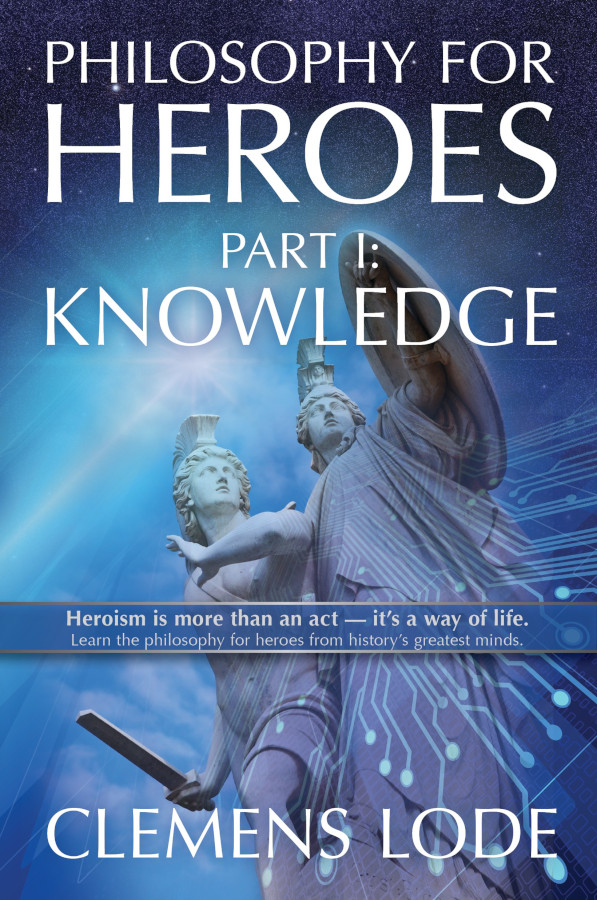
\includegraphics{images/P4H_Cover_12-10-16-front-900.jpg}~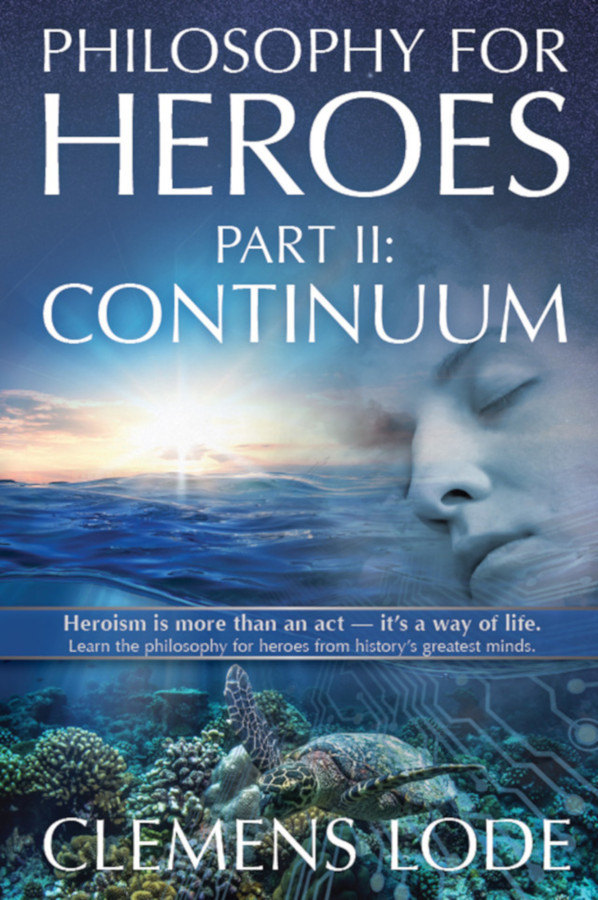
\includegraphics{images/pfh2-cover-900.jpg}
\label{c1_pfh:fig}
\end{figure}

\begin{figure}[H]\centering

\includegraphics{images/Agile_5-11-17_HiRes2-900.jpg}~
\includegraphics{images/KanbanFront_6-28-17_HiRes-900.jpg}
\label{c1_projectmanagement:fig}
\end{figure}

% Remove the following section if you only want to show your covers, replace with your own book descriptions. The example entries are books I have written using this template.


Here are other books by YOUR NAME. All share the topics of philosophy, psychology, leadership, and project management.

\begin{setlength}{\leftmargin}{1cm} 
\begin{description}\setlength{\itemsep}{-5pt}

\item[Better Books with LaTeX] In \citetitle{BBWL}\index{@\citetitle{BBWL}}\ifxetex\else \citep{BBWL}\fi, author Clemens Lode provides you a short-cut into the world of book publishing with \LaTeX{}. It is not a book that just lists all the commands and then leave you alone, it guides you alongside a fully working template (this one!).

\item[Part I: Knowledge.] In \citetitle{PFH1E}\index{@\citetitle{PFH1E}}, the first book in this four-book series, author Clemens Lode takes the reader on a journey, examining the foundations of knowledge. What is the basis of our understanding of the world? How does society define a ``hero''? How do basic skills, such as language and mathematics, train our way of thinking and reasoning?

\item[Part II: Continuum.] Beyond the static world of the first book, \citetitle{PFH2E}\index{@\citetitle{PFH2E}} looks at gradual transitions from one condition to the next. Where do we come from? Why is there something rather than nothing? What is the source of our creativity? How can the study of natural sciences help us to understand who we are?

\item[Scrum Your Jira!] In \citetitle{scrum-your-jira}\index{@\citetitle{scrum-your-jira}}\ifxetex\else \citep{scrum-your-jira}\fi, author Clemens Lode challenges two illusions that can get in the way of your company's road to being truly Agile: first, that your Scrum is ``special,'' and second, that you can hide behind project management software. Jira is powerful\emdash{}and this book will show you how to use it more effectively\emdash{}but it makes it easy to forget that the first idea of Agile is: Individuals and interactions over processes and tools.

\item[Kanban Remastered] StarCraft, the most popular real-time strategy game of all time, is also all about producing and deploying just as many game units at just the right time. This book is about the relationship of StarCraft and Kanban. When your team knows StarCraft but not Kanban, \citetitle{kanban-remastered}\index{@\citetitle{kanban-remastered}}\ifxetex\else \citep{kanban-remastered}\fi will provide you with a series of analogies to allow a better and easier understanding of Agile principles. It is written in a light-hearted tone, similar to how you might chat with a fellow coach about your Agile experiences implementing Kanban, taking for granted that you have experience with StarCraft.

\end{description}
\end{setlength}\blankpage

% list of uncited references that are still good reads (only for printed PDF)
\ifxetex
	%%%%%%%%%%%%%%%%%%%%%%%%%%%%%%%%%%%%%
% Read the /ReadMeFirst/ReadMeFirst.tex for an introduction. Check out the accompanying book "Better Books with LaTeX" for a discussion of the template and step-by-step instructions. The template was originally created by Clemens Lode, LODE Publishing (www.lode.de), mail@lode.de, 8/17/2018. Feel free to use this template for your book project!
%%%%%%%%%%%%%%%%%%%%%%%%%%%%%%%%%%%%%

% list of uncited references that are still good reads (only for printed PDF). Replace the citations accordingly.

\nocite{PFH1E}
\nocite{PFH2E}
\nocite{PFH3E}
\nocite{PFH4E}

\printbibliography[keyword=recommendedEN, title={Recommended Reading}]\blankpage
\fi

%%%%%%%%%%%%%%%%%%%%%%%%%%%%%%%%%%%%%
% Read the /ReadMeFirst/ReadMeFirst.tex for an introduction. Check out the accompanying book "Better Books with LaTeX" for a discussion of the template and step-by-step instructions. The template was originally created by Clemens Lode, LODE Publishing (www.lode.de), mail@lode.de, 8/17/2018. Feel free to use this template for your book project!
%%%%%%%%%%%%%%%%%%%%%%%%%%%%%%%%%%%%%


% Upload hires (author_highres.png) and lowres picture (author.jpg) of author into images folder, and uncomment the 5 includegraphics lines.
% Replace quotation text
% Add text describing your motivation, your professional background, what you are currently doing, and how to connect with you.

\begin{chapterpage}{
	{The Author}
}{p1_the-author:cha}

\vspace*{\fill}

\begin{center}

%\ifxetex
%	\includegraphics[width=.7\textwidth]{images/author_hires.png}
%\else
%	\includegraphics{images/author.jpg}
%\fi

\end{center}
\vspace*{\fill}

\begin{myquotation} Here is space for a quotation that describes your journey through life (as opposed to just during the writing of this book). Pick one that best describes you, your attitude, or something you admire. Be personal!\end{myquotation}

\end{chapterpage}

Describe your dreams, what goals you have in life, where you went to school or studied, and what job you currently work or worked in the past. Make clear what motivated you to start writing. Finally, add contact points where people can connect with you (mail, Facebook, Twitter, etc.). 
\blankpage
%%%%%%%%%%%%%%%%%%%%%%%%%%%%%%%%%%%%%
% Read the /ReadMeFirst/ReadMeFirst.tex for an introduction. Check out the accompanying book "Better Books with LaTeX" for a discussion of the template and step-by-step instructions. The template was originally created by Clemens Lode, LODE Publishing (www.lode.de), mail@lode.de, 8/17/2018. Feel free to use this template for your book project!
%%%%%%%%%%%%%%%%%%%%%%%%%%%%%%%%%%%%%

% Use this chapter to summarize what you have learned while writing the book. This helps you to write better books in the future and might be interesting for the reader to know about how the book came about.

\begin{chapterpage}{The Book's Story}{p2_booksstory:cha}

% Add a quotation to set the team for your lessons learned

\end{chapterpage}



\blankpage


% switch back to basic chapter design
%  Reset the chapter design to a basic one (no box, just underlined chapter title---used for the back and front matter)

\renewcommand*\chapterheadstartvskip{\vspace*{-3\topskip}} 
\renewcommand*\chapterheadendvskip{
  \vskip-.5\baselineskip
  \noindent
  {\color{gray}\rule{\linewidth}{2pt}}
  \par}
\renewcommand*\chapterformat{}
\renewcommand*{\chapterpagestyle}{empty}

% needs to be in curly braces because parskip change.
{
\parskip=5pt
%%%%%%%%%%%%%%%%%%%%%%%%%%%%%%%%%%%%%
% Read the /ReadMeFirst/ReadMeFirst.tex for an introduction. Check out the accompanying book "Better Books with LaTeX" for a discussion of the template and step-by-step instructions. The template was originally created by Clemens Lode, LODE Publishing (www.lode.de), mail@lode.de, 8/17/2018. Feel free to use this template for your book project!
%%%%%%%%%%%%%%%%%%%%%%%%%%%%%%%%%%%%%

\chapter{Reflection}

\begin{problem}
Introductory text about what this section is about. For example, describe that this is a summary of all the problem boxes throughout the book and point to an online forum where readers can discuss them.\end{problem}

% Reset formatting
\setlength{\parindent}{0.0cm}
\renewcommand{\index}[1]{}
\renewenvironment{problem}[1][]{$\bullet$\ #1}
\footnotesize 


\section*{Replace with Your First Chapter}
% Add questions located in your first chapter.
\begin{problem}What is LaTeX?\end{problem}


\section*{Replace with Your Second Chapter}
% Add questions located in your second chapter.
\begin{problem}What is LaTeX?\end{problem}


\section*{Replace with Your Third Chapter}
% Add questions located in your third chapter.
\begin{problem}What is LaTeX?\end{problem}
\newpage
%%%%%%%%%%%%%%%%%%%%%%%%%%%%%%%%%%%%%
% Read the /ReadMeFirst/ReadMeFirst.tex for an introduction. Check out the accompanying book "Better Books with LaTeX" for a discussion of the template and step-by-step instructions. The template was originally created by Clemens Lode, LODE Publishing (www.lode.de), mail@lode.de, 8/17/2018. Feel free to use this template for your book project!
%%%%%%%%%%%%%%%%%%%%%%%%%%%%%%%%%%%%%

\chapter{Eureka!}

\begin{idea}
Introductory text about what this section is about. For example, describe that this is a summary of all the idea boxes throughout the book.\end{idea}

% reformat idea boxes
\renewenvironment{idea}[1][]{$\bullet$\ #1}
%\setlength{\parindent}{0.7cm}

% deactivate indexing of idea boxes to prevent duplicates
\ifxetex
	\renewcommand{\index}{}
\fi

\section*{Replace with Your First Chapter}
% Add ideas located in your first chapter.
\begin{idea}
\LaTeX{} is a document preparation system.
\end{idea}

\section*{Replace with Your Second Chapter}
% Add ideas located in your second chapter.
\begin{idea}
\LaTeX{} is a document preparation system.
\end{idea}

\section*{Replace with Your Third Chapter}
% Add ideas located in your third chapter.
\begin{idea}
\LaTeX{} is a document preparation system.
\end{idea}\newpage
\parskip=0pt
%%%%%%%%%%%%%%%%%%%%%%%%%%%%%%%%%%%%%
% Read the /ReadMeFirst/ReadMeFirst.tex for an introduction. Check out the accompanying book "Better Books with LaTeX" for a discussion of the template and step-by-step instructions. The template was originally created by Clemens Lode, LODE Publishing (www.lode.de), mail@lode.de, 8/17/2018. Feel free to use this template for your book project!
%%%%%%%%%%%%%%%%%%%%%%%%%%%%%%%%%%%%%


% If you have added or removed any entries in the glossary directory, add them here. If a letter is missing, add a new \section*{} with the letter.

\chapter{Glossary}

% Special formatting for glossary 
\setlength{\parindent}{0.7cm}
\renewcommand{\index}[1]{}
\renewenvironment{definition}[2][]{\textbf{#2}\ $\bullet$\ #1}
\footnotesize
\ifxetex
	\titlespacing*{\section}{0pt}{3.5ex plus 1ex minus .2ex}{2.3ex plus .2ex}
\fi

\vspace{20pt}


\section*{E}
\begin{multicols}{2}
\begin{definition}{Entity}\index{entity|textbf} An \emph{entity} is a ``thing'' with properties (an identity). For example, a plant produces oxygen, a stone has a hard surface, etc.).\end{definition}
\end{multicols}

\section*{I}
\begin{multicols}{2}
\begin{definition}{Identity}\index{identity|textbf} An \emph{identity} is the sum total of all properties\index{entity!property} of an entity (e.g., weight: 160 pounds, length: 6 feet, has a consciousness, etc.).\end{definition}

\end{multicols}

\section*{L}
\begin{multicols}{2}
\begin{definition}{LaTeX}\index{latex|textbf} \LaTeX{} is a document preparation system.\end{definition}
\end{multicols}

\section*{P}
\begin{multicols}{2}
\begin{definition}{Property}\index{entity!property|textbf} A \emph{property} refers to the manner in which an entity (or a process) affects other entities (or other processes) in a certain situation (e.g., mass, position, length, name, velocity, etc.).\end{definition}
\end{multicols}\newpage
% add separate quotations page (sources in the e-book are already included in the text body)
\ifxetex
	%%%%%%%%%%%%%%%%%%%%%%%%%%%%%%%%%%%%%
% Read the /ReadMeFirst/ReadMeFirst.tex for an introduction. Check out the accompanying book "Better Books with LaTeX" for a discussion of the template and step-by-step instructions. The template was originally created by Clemens Lode, LODE Publishing (www.lode.de), mail@lode.de, 8/17/2018. Feel free to use this template for your book project!
%%%%%%%%%%%%%%%%%%%%%%%%%%%%%%%%%%%%%

% quotation sources (only for print PDF where the source is not directly mentioned in the text body).

\chapter{Quotation Sources}

\setlength{\parindent}{0pt}
\footnotesize

\babelDE{\textbf{\pageref{gogh-sky-quote}:} \cite[vgl.][S.~23--24]{ifyouwanttowrite}}
\babelEN{\textbf{\pageref{gogh-sky-quote}:} \cite[pp.~23--24]{ifyouwanttowrite}}\par
\fi
}

%%%%%%%%%%%%%%%%%%%%%%%%%%%%%%%%%%%%%
% Read the /ReadMeFirst/ReadMeFirst.tex for an introduction. Check out the accompanying book "Better Books with LaTeX" for a discussion of the template and step-by-step instructions. The template was originally created by Clemens Lode, LODE Publishing (www.lode.de), mail@lode.de, 8/17/2018. Feel free to use this template for your book project!
%%%%%%%%%%%%%%%%%%%%%%%%%%%%%%%%%%%%%


% Command to add some text into the bibliography (between the title and the list of referenced books)
% See https://tex.stackexchange.com/questions/197061/text-between-index-or-bibliography-title-and-content
\newcommand{\bibpreface}[1]{\patchcmd{\thebibliography}{\list}{#1\list}{}{}}

\bibpreface{Write here the preface of your list of recommended reading titles. Delete this line to have no preface for this section.}

\ifxetex
	\printbibliography
\else
	\newpage
	\bibliographystyle{plainnat}
	\bibliography{bibliography/english}
\fi


% ---------- Appendix
\appendix
    
%%%%%%%%%%%%%%%%%%%%%%%%%%%%%%%%%%%%%
% Read the /ReadMeFirst/ReadMeFirst.tex for an introduction. Check out the accompanying book "Better Books with LaTeX" for a discussion of the template and step-by-step instructions. The template was originally created by Clemens Lode, LODE Publishing (www.lode.de), mail@lode.de, 8/17/2018. Feel free to use this template for your book project!
%%%%%%%%%%%%%%%%%%%%%%%%%%%%%%%%%%%%%

% the index page, only for printed PDF

\ifxetex	
	\pagestyle{empty}
	\appendix
	\indexprologue{Replace index prologue with an own introduction of how to contact you when there is an errata concerning the index.}
    \printindex
\fi

%%%%%%%%%%%%%%%%%%%%%%%%%%%%%%%%%%%%%
% Read the /ReadMeFirst/ReadMeFirst.tex for an introduction. Check out the accompanying book "Better Books with LaTeX" for a discussion of the template and step-by-step instructions. The template was originally created by Clemens Lode, LODE Publishing (www.lode.de), mail@lode.de, 8/17/2018. Feel free to use this template for your book project!
%%%%%%%%%%%%%%%%%%%%%%%%%%%%%%%%%%%%%


% Replace it with your own call to action if you like, or use the default text.

\chapter{An Important Final Note}

% Only show for e-books.
\ifxetex \else \textit{If you want to rate this e-book, please also add a short text comment. Without a text comment, your star rating will be invisible on the Amazon website and count only as an indicator for further recommendations on Amazon. Thanks!}\fi

Writers are not performance artists. While there are book signings and public readings, most writers (and readers) follow their passion alone in their homes.

\textit{What applause is for the musician, \textbf{reviews} are for the writer.} 

\textit{Books create a community among readers}; you can share your thoughts among all those who will or have read the book.

\textbf{Leave a thoughtful honest review and help me to create such a community on the platform on which you have acquired this book.} \textit{What did you like, what can be improved? To whom would you recommend it?} 

Thank you, also in the name of all the other readers who will be able to better decide whether this book is right for them or not! A positive review will increase the reach of the book, a negative review will improve the quality of the next book. I welcome both!
%%%%%%%%%%%%%%%%%%%%%%%%%%%%%%%%%%%%%
% Read the /ReadMeFirst/ReadMeFirst.tex for an introduction. Check out the accompanying book "Better Books with LaTeX" for a discussion of the template and step-by-step instructions. The template was originally created by Clemens Lode, LODE Publishing (www.lode.de), mail@lode.de, 8/17/2018. Feel free to use this template for your book project!
%%%%%%%%%%%%%%%%%%%%%%%%%%%%%%%%%%%%%

% Replace quote

\newpage
\thispagestyle{empty}
\vspace*{\fill}
\hfill

\babelEN{\begin{myquotation} Replace this quote\par\mbox{}\hfill \emdash{}Name of the author\end{myquotation}}

\end{document}